\subsection{Carbon-aware computing}
\label{subsec:carbon_aware_computing}

Le sottosezioni precedenti hanno analizzato approcci che perseguono la
sostenibilità energetica dell'elaborazione serverless operando su due
leve distinte: la scelta del nodo di esecuzione (scheduling
energy-aware) e la modulazione della logica applicativa (approximate
computing). In entrambi i casi, il criterio di ottimizzazione è il
consumo energetico in sé: l'obiettivo è ridurre i Joule consumati per
invocazione o rispettare un budget energetico prefissato,
indipendentemente dal momento in cui tale consumo avviene.

Questa impostazione non cattura una dimensione rilevante del problema:
come discusso nella Sezione~\ref{subsec:carbon_intensity}, l'impatto
ambientale di un'unità di energia consumata non è costante, ma dipende
dalla carbon intensity della rete elettrica nel momento e nel luogo
dell'esecuzione. Il paradigma del \emph{carbon-aware computing} si
fonda su questa osservazione: anziché trattare ogni kilowattora come
equivalente, le decisioni di esecuzione possono essere modulate in
funzione della carbon intensity corrente, spostando il criterio di
ottimizzazione dal solo consumo energetico all'impatto ambientale
complessivo dell'esecuzione.

In letteratura, le strategie carbon-aware sono state declinate
attraverso due leve principali. La prima, denominata \emph{temporal
shifting}, consiste nel posticipare l'esecuzione di carichi di lavoro
tolleranti al ritardo verso momenti in cui la carbon intensity della
rete locale è prevista più bassa. La seconda, denominata \emph{spatial
shifting}, consiste nel distribuire i carichi di lavoro tra data center
situati in regioni geografiche con diversi livelli di carbon intensity,
privilegiando l'esecuzione nei siti con il mix energetico più
favorevole al momento dell'invocazione. Entrambe le strategie
presuppongono la disponibilità di dati sulla carbon intensity in tempo
reale o tramite previsioni a breve termine, tipicamente forniti da
servizi specializzati quali ElectricityMaps~\cite{electricitymaps2024}
o WattTime.

Nei paragrafi seguenti vengono analizzati due contributi che
rappresentano queste direzioni in contesti distinti: il
\emph{Carbon-Intelligent Computing System} (CICS) di
Google~\cite{radovanovic2022carbon}, che costituisce il primo sistema
carbon-aware in produzione su scala industriale e opera attraverso
temporal shifting di workload batch nei data center; e
GreenCourier~\cite{greencourier}, che porta il paradigma carbon-aware
specificamente nel contesto delle piattaforme FaaS/serverless,
adottando una strategia di spatial shifting per la schedulazione delle
funzioni tra regioni geografiche distribuite.

% ── Google CICS ────────────────────────────────────────────────────────
 
\subsubsection{Temporal shifting su scala industriale: il Carbon-Intelligent Computing System}
\label{subsubsec:google_cics}
 
Il \emph{Carbon-Intelligent Computing System}
(CICS)~\cite{radovanovic2022carbon}, sviluppato e operato da Google,
rappresenta il primo sistema carbon-aware implementato in produzione su
scala globale. Il sistema opera su oltre 20 data center distribuiti in
4 continenti e gestisce un consumo elettrico superiore a 15,5 terawattora
annui, rendendolo il caso di studio di riferimento per l'applicazione
del carbon-aware computing a infrastrutture di calcolo reali.
 
Il problema affrontato dal CICS può essere descritto in termini
intuitivi. I data center di Google eseguono due tipologie di carichi di
lavoro con caratteristiche temporali molto diverse. La prima comprende i
servizi rivolti agli utenti --- ricerca, mappe, streaming --- e le
macchine virtuali dei clienti cloud: questi carichi sono
\emph{inflexible}, nel senso che devono essere eseguiti nel momento in
cui vengono richiesti, senza possibilità di posticipazione. La seconda
tipologia comprende processi batch --- compressione dei dati,
addestramento di modelli di machine learning, pipeline di elaborazione
video --- che tollerano ritardi purché il lavoro venga completato entro
24 ore: questi carichi sono \emph{flexible}. Il CICS sfrutta la
flessibilità temporale di questa seconda categoria: se la carbon
intensity della rete elettrica locale è alta in un determinato momento
della giornata, il sistema riduce la quantità di lavoro batch ammesso
in quel momento, accumulandolo per eseguirlo nelle ore successive in
cui la rete è alimentata da fonti più pulite. Il volume complessivo di
lavoro giornaliero non cambia --- viene soltanto redistribuito nel tempo
per allinearlo al profilo della carbon intensity.
 
Il meccanismo con cui il CICS realizza questa redistribuzione è la
\emph{Virtual Capacity Curve} (VCC). Per ciascun cluster di calcolo, il
sistema genera giornalmente una curva che definisce, ora per ora, il
limite massimo di risorse computazionali disponibili per i workload
flessibili nel giorno successivo. Questa curva non è uniforme: nelle
ore in cui la carbon intensity è prevista alta, il limite viene
abbassato, impedendo allo scheduler dei job (Borg) di ammettere nuovi
job batch; nelle ore con carbon intensity bassa, il limite viene alzato,
consentendo l'esecuzione del lavoro accumulato. Il risultato, illustrato
in Figura~\ref{fig:vcc_mechanism}, è uno spostamento del carico
flessibile dalle ore centrali della giornata --- tipicamente
caratterizzate da carbon intensity più elevata --- verso le prime ore
del mattino e la sera, quando la rete tende ad essere più pulita.
 
\begin{figure}[ht]
    \centering
    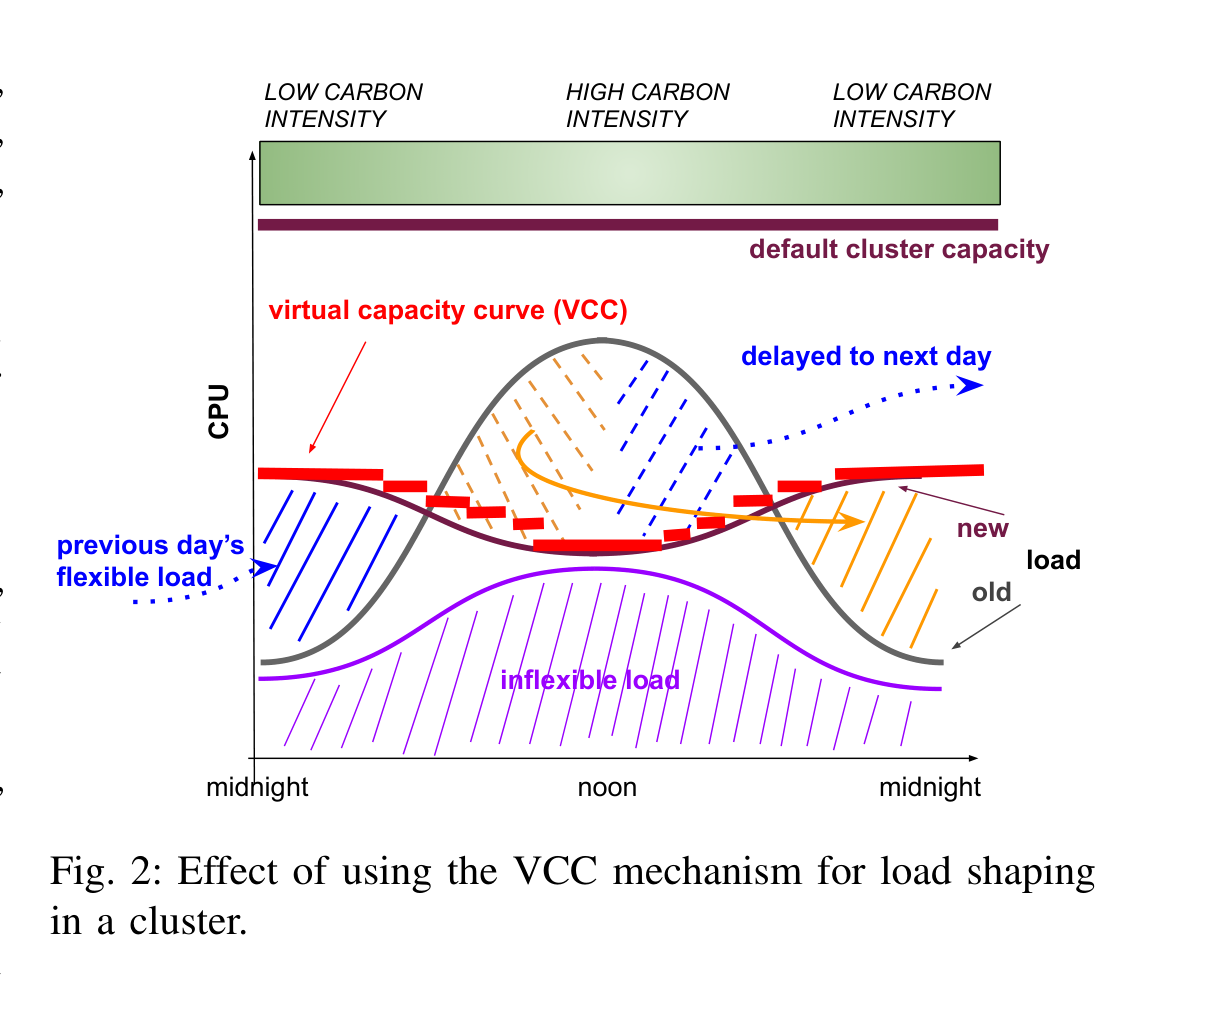
\includegraphics[width=0.85\textwidth]{figures/vcc_mechanism.png}
    \caption{Effetto della Virtual Capacity Curve (VCC) sul profilo di
    carico di un cluster. La barra superiore indica i livelli di carbon
    intensity nel corso della giornata. La curva VCC (in rosso) riduce la
    capacità disponibile per i workload flessibili nelle ore ad alta
    carbon intensity, spostando il carico (aree arancione e blu) verso
    le ore più pulite della giornata. Il carico inflexible (in viola)
    non viene alterato.}
    \label{fig:vcc_mechanism}
\end{figure}
 
È importante osservare che la VCC non interviene sui singoli job: non
decide quali job eseguire o in quale ordine, né modifica la logica dei
job stessi. La VCC agisce a un livello superiore, impostando un vincolo
aggregato sulla quantità totale di risorse disponibili per i workload
flessibili in ciascuna ora. Lo scheduler dei job (Borg) continua a
operare normalmente entro questo vincolo, senza necessità di
modifiche: se la capacità disponibile è ridotta, semplicemente meno job
vengono ammessi e quelli in attesa rimangono in coda fino a quando la
capacità non viene ripristinata.
 
I valori orari della VCC sono calcolati giornalmente attraverso un
processo di ottimizzazione che utilizza previsioni di domanda per i
workload flessibili e inflexible, modelli di traduzione dell'utilizzo
CPU in consumo elettrico, e previsioni di carbon intensity oraria
fornite da ElectricityMaps~\cite{electricitymaps2024} per ciascuna zona
della rete in cui risiedono i data center.
 
I risultati operativi riportati dagli autori mostrano che, nei cluster
in cui il CICS è attivo, il consumo di potenza si riduce dell'1--2\%
nelle ore con la carbon intensity più alta rispetto ai cluster non
ottimizzati.
 
Dal punto di vista concettuale, il CICS stabilisce il principio
fondamentale del carbon-aware computing: la carbon intensity della rete
elettrica può essere utilizzata come segnale operativo per modulare le
decisioni di esecuzione, trasformando l'ottimizzazione del consumo
energetico in un'ottimizzazione dell'impatto ambientale. È opportuno
osservare, tuttavia, che il sistema opera esclusivamente attraverso
temporal shifting di workload batch tolleranti al ritardo, su orizzonti
temporali di 24 ore e a granularità di cluster. Non considera la
possibilità di agire sulla logica applicativa dei workload né di
selezionare tra varianti di esecuzione con profili diversi. Inoltre, il
contesto operativo --- data center hyperscale con job batch --- è
significativamente diverso da quello delle piattaforme FaaS, dove le
funzioni sono invocate su richiesta con requisiti di latenza stringenti.
 
% ── GreenCourier ───────────────────────────────────────────────────────

\subsubsection{Spatial shifting carbon-aware per funzioni serverless}
\label{subsubsec:greencourier}

Se il CICS affronta il carbon-aware computing attraverso il temporal
shifting di workload batch in data center hyperscale,
GreenCourier~\cite{greencourier} porta il paradigma nel contesto
specifico delle piattaforme serverless, adottando una strategia di
spatial shifting: anziché posticipare l'esecuzione nel tempo, il
sistema distribuisce le invocazioni delle funzioni tra cluster
Kubernetes situati in regioni geografiche diverse, privilegiando
l'esecuzione nella regione con la carbon intensity marginale più bassa
al momento dell'invocazione.

Come illustrato in Figura~\ref{fig:greencourier_arch}, il framework si
integra con la piattaforma serverless Knative e si articola in tre
componenti principali. Il \emph{Metrics Server} raccoglie e normalizza
in tempo reale i punteggi di carbon intensity per ciascuna regione
geografica, utilizzando come fonti dati servizi quali WattTime o il
Carbon-aware SDK della Green Software Foundation. Lo scheduler custom,
implementato come plugin di scoring nel framework di scheduling di
Kubernetes, assegna a ciascun nodo candidato un punteggio proporzionale
alla carbon efficiency della regione in cui è localizzato.
L'infrastruttura multi-cluster, realizzata tramite Liqo, consente il
\emph{peering} tra cluster indipendenti distribuiti geograficamente e
l'offloading trasparente delle funzioni verso regioni remote.

\begin{figure}[ht]
    \centering
    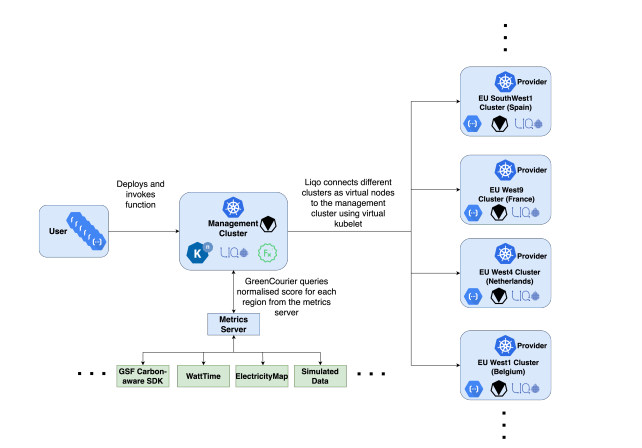
\includegraphics[width=0.9\textwidth]{figures/Greencourier architecture.png}
    \caption{Architettura di GreenCourier. Il management cluster ospita
    lo scheduler carbon-aware e il Metrics Server, che interroga sorgenti
    di carbon intensity (WattTime, ElectricityMaps). I provider cluster,
    distribuiti in diverse regioni europee, sono collegati tramite Liqo
    come nodi virtuali. Lo scheduler assegna ciascuna invocazione alla
    regione con la carbon intensity più favorevole.}
    \label{fig:greencourier_arch}
\end{figure}

Il meccanismo decisionale opera per ciascuna invocazione: quando una
funzione viene sottomessa, lo scheduler interroga il Metrics Server per
ottenere i punteggi di carbon intensity correnti delle regioni
disponibili, normalizza i valori e seleziona il nodo con il punteggio
più favorevole. I punteggi vengono aggiornati con una granularità di
cinque minuti, coerente con la frequenza di aggiornamento dei dati
forniti dalle sorgenti di carbon intensity, e mantenuti in cache locale
per ridurre l'overhead di comunicazione durante lo scheduling.

I risultati sperimentali, condotti su Google Kubernetes Engine con
cluster distribuiti tra Spagna, Francia, Belgio e Paesi Bassi e
utilizzando tracce di invocazione reali da Azure Functions, mostrano che
GreenCourier riduce le emissioni di carbonio per invocazione in media
del 13,25\% rispetto alla strategia di scheduling predefinita di
Kubernetes e del 17,8\% rispetto a una strategia basata sulla
prossimità geografica. Questo risultato è ottenuto al costo di un
incremento medio del 10,26\% nei tempi di risposta delle funzioni,
dovuto all'esecuzione in regioni geograficamente più distanti ma con
carbon intensity più favorevole.

Dal punto di vista della relazione con il contesto analizzato in questo
capitolo, GreenCourier è il primo lavoro che applica il paradigma
carbon-aware specificamente allo scheduling di funzioni serverless. A
differenza del CICS, che opera su workload batch con flessibilità
temporale, GreenCourier gestisce invocazioni on-demand con requisiti di
risposta immediata, dimostrando che il spatial shifting carbon-aware è
applicabile anche in contesti con vincoli di latenza.

% ── Osservazioni conclusive ────────────────────────────────────────────

\vspace{0.5em}

I due contributi analizzati in questa sottosezione introducono la carbon
intensity della rete elettrica come segnale di contesto per le decisioni
di esecuzione, estendendo il criterio di ottimizzazione dal solo consumo
energetico all'impatto ambientale complessivo. Entrambi gli approcci
condividono tuttavia una caratteristica comune con le famiglie di
soluzioni esaminate nelle sottosezioni precedenti: la carbon intensity
viene utilizzata per decidere \emph{dove} o \emph{quando} eseguire un
carico di lavoro, ma la funzione eseguita rimane invariante rispetto
alle condizioni della rete elettrica, senza che il segnale ambientale
orienti la selezione tra varianti con profili energia-accuratezza
differenziati.